\documentclass[a4paper,twoside]{article}
\usepackage[T1]{fontenc}
\usepackage[bahasa]{babel}
\usepackage{graphicx}
\graphicspath{ {img/} }
\usepackage{graphics}
\usepackage{float}
\usepackage[cm]{fullpage}
\pagestyle{myheadings}
\usepackage{etoolbox}
\usepackage{setspace} 
\usepackage{lipsum} 
\usepackage{listings}
\usepackage{wrapfig}
\setlength{\headsep}{30pt}
\usepackage[inner=2cm,outer=2.5cm,top=2.5cm,bottom=2cm]{geometry} %margin
% \pagestyle{empty}

\makeatletter
\renewcommand{\@maketitle} {\begin{center} {\LARGE \textbf{ \textsc{\@title}} \par} \bigskip {\large \textbf{\textsc{\@author}} }\end{center} }
\renewcommand{\thispagestyle}[1]{}
\markright{\textbf{\textsc{Laporan Perkembangan Pengerjaan Skripsi\textemdash Sem. Ganjil 2017/2018}}}

\onehalfspacing
 
\begin{document}

\title{\@judultopik}
\author{\nama \textendash \@npm} 

%ISILAH DATA BERIKUT INI:
\newcommand{\nama}{Nancy Valentina}
\newcommand{\@npm}{2014730049}
\newcommand{\tanggal}{23/11/2017} %Tanggal pembuatan dokumen
\newcommand{\@judultopik}{Aplikasi Pratinjau 3 Dimensi Berbasis Web} % Judul/topik anda
\newcommand{\kodetopik}{PAN4304}
\newcommand{\jumpemb}{1} % Jumlah pembimbing, 1 atau 2
\newcommand{\pembA}{Pascal Alfadian Nugroho}
\newcommand{\pembB}{-}
\newcommand{\semesterPertama}{43 - Ganjil 17/18} % semester pertama kali topik diambil, angka 1 dimulai dari sem Ganjil 96/97
\newcommand{\lamaSkripsi}{1} % Jumlah semester untuk mengerjakan skripsi s.d. dokumen ini dibuat
\newcommand{\kulPertama}{Skripsi 1} % Kuliah dimana topik ini diambil pertama kali
\newcommand{\tipePR}{B} % tipe progress report :
% A : dokumen pendukung untuk pengambilan ke-2 di Skripsi 1
% B : dokumen untuk reviewer pada presentasi dan review Skripsi 1
% C : dokumen pendukung untuk pengambilan ke-2 di Skripsi 2

% Dokumen hasil template ini harus dicetak bolak-balik !!!!

\maketitle

\pagenumbering{arabic}

\section{Data Skripsi} %TIDAK PERLU MENGUBAH BAGIAN INI !!!
Pembimbing utama/tunggal: {\bf \pembA}\\
Pembimbing pendamping: {\bf \pembB}\\
Kode Topik : {\bf \kodetopik}\\
Topik ini sudah dikerjakan selama : {\bf \lamaSkripsi} semester\\
Pengambilan pertama kali topik ini pada : Semester {\bf \semesterPertama} \\
Pengambilan pertama kali topik ini di kuliah : {\bf \kulPertama} \\
Tipe Laporan : {\bf \tipePR} -
\ifdefstring{\tipePR}{A}{
			Dokumen pendukung untuk {\BF pengambilan ke-2 di Skripsi 1} }
		{
		\ifdefstring{\tipePR}{B} {
				Dokumen untuk reviewer pada presentasi dan {\bf review Skripsi 1}}
			{	Dokumen pendukung untuk {\bf pengambilan ke-2 di Skripsi 2}}
		}

\section{Detail Perkembangan Pengerjaan Skripsi}
Detail bagian pekerjaan skripsi sesuai dengan rencan kerja/laporan perkembangan terkahir :
	\begin{enumerate}
		\item \textbf{Mempelajari standar WebGL sebagai \textit{\textbf{Application Programming Interface}} untuk menampilkan grafis 3
dimensi pada \textit{\textbf{web browser}}).}\\
		{\bf Status :} Ada sejak rencana kerja skripsi.\\
		{\bf Hasil :} Berikut ini merupakan hasil dari pembelajaran standar WebGL sebagai \textit{Application Programming Interface} untuk menampilkan grafis 3 dimensi pada web {\it browser}:

WebGL adalah sebuah Application Programming Interface (API) yang membangun objek 3 dimensi dengan mode langsung yang dirancang untuk {\it web}. WebGL diturunkan dari OpenGL ES 2.0, WebGL menyediakan fungsi pembangunan sejenis tetapi di dalam konteks HTML. WebGL dirancang sebagai konteks pembangunan objek pada elemen {\it canvas} HTML. {\it Canvas} pada HTML menyediakan suatu destinasi untuk pembangunan objek secara programatik pada halaman {\it web} dan memungkinkan menampilkan objek yang sedang dibangun menggunakan API pembangun objek yang berbeda. Berikut ini merupakan {\it interfaces} dan fungsionalitas yang ada pada WebGL:
\begin{enumerate}
\item {\it WebGLObject}

	{\it Interface WebGLObject} merupakan {\it interface} awal untuk diturunkan kepada semua objek GL.
	\begin{lstlisting}[caption={{\it Interface} awal pada WebGL.}, captionpos=b]
interface WebGLObject {
};
	\end{lstlisting}
	
\item {\it WebGLFrameBuffer}

	{\it Interface WebGLFrameBuffer} merepresentasikan sebuah OpenGL {\it Frame Buffer Object}.
	\begin{lstlisting}[caption={{\it Frame Buffer Object} pada OpenGL.}, captionpos=b]
interface WebGLFramebuffer : WebGLObject {
};
	\end{lstlisting}

\item {\it WebGLProgram}

	{\it Interface WebGLProgram} merepresentasikan sebuah OpenGL {\it Program Object}.
	\begin{lstlisting}[caption={{\it Program Object} pada OpenGL.}, captionpos=b]
interface WebGLProgram : WebGLObject {
};
	\end{lstlisting}
	
 {\it WebGLShader}

	{\it Interface WebGLShader} merepresentasikan sebuah OpenGL {\it Shader Object}.
	\begin{lstlisting}[caption={{\it Shader Object} pada OpenGL.}, captionpos=b]
interface WebGLShader : WebGLObject {
};
	\end{lstlisting}

\item {\it WebGLTexture}

	{\it Interface WebGLTexture} merepresentasikan sebuah OpenGL {\it Texture Object}.
	\begin{lstlisting}[caption={{\it Texture Object} pada OpenGL.}, captionpos=b]
interface WebGLTexture : WebGLObject {
};
	\end{lstlisting}
\item {\it ArrayBuffer} dan {\it Typed Arrays}

	{\it Vertex, index, texture,} dan data lainnya ditransfer ke implementasi WebGL menggunakan {\it ArrayBuffer, Typed Arrays,} dan {\it DataViews} seperti yang telah didefinisikan pada spesifikasi ECMAScript.
\begin{lstlisting}[caption={Transfer data ke implementasi WebGL.}, captionpos=b]
var numVertices = 100; // for example

// Hitung ukuran buffer yang dibutuhkan dalam bytes dan floats
var vertexSize = 3 * Float32Array.BYTES_PER_ELEMENT +
4 * Uint8Array.BYTES_PER_ELEMENT;
var vertexSizeInFloats = vertexSize / Float32Array.BYTES_PER_ELEMENT;

// Alokasikan buffer
var buf = new ArrayBuffer(numVertices * vertexSize);

// Map buffer ke Float32Array untuk mengakses posisi
var positionArray = new Float32Array(buf);

	// Map buffer yang sama ke Uint8Array untuk mengakses warna
var colorArray = new Uint8Array(buf);

// Inisialisasi offset dari vertices dan warna pada buffer
var positionIdx = 0;
var colorIdx = 3 * Float32Array.BYTES_PER_ELEMENT;

// Inisialisasi buffer
for (var i = 0; i < numVertices; i++) {
    	positionArray[positionIdx] = ...;
    	positionArray[positionIdx + 1] = ...;
    	positionArray[positionIdx + 2] = ...;
    	colorArray[colorIdx] = ...;
    	colorArray[colorIdx + 1] = ...;
    	colorArray[colorIdx + 2] = ...;
    	colorArray[colorIdx + 3] = ...;
   	positionIdx += vertexSizeInFloats;
   	colorIdx += vertexSize;
}
\end{lstlisting}
	
\item {\it WebGL Contect}
	{\it WebGLRenderingContext} merepresentasikan API yang memungkinkan gaya pembangunan OpenGL ES 2.0 ke elemen {\it canvas}.

\item {\it WebGLContextEvent}
	WebGL menghasilkan sebuah {\it WebGLContextEvent} sebagai respon dari perubahan penting pada status konteks pembangunan WebGL. {\it Event} tersebut dikirim melalui {\it DOM Event System} dan dilanjutkan ke HTMLCanvasEvent yang diasosiasikan dengan konteks pembangunan WebGL.

\end{enumerate}
		
		\item \textbf{Mempelajari penggunaan pustaka Three.js sebagai pustaka perantara untuk penggunaan WebGL.}\\
		{\bf Status :} Ada sejak rencana kerja skripsi.\\
		{\bf Hasil :} Berikut ini merupakan hasil dari pembelajaran Three.js sebagai pustaka perantara untuk penggunaan WebGL:
		
Pustaka Three.js ini bertujuan untuk membuat pustaka 3 dimensi yang mudah dan ringan untuk digunakan. Pustaka ini menyediakan <canvas>, <svg>, CSS3D, dan pembangun WebGL.
Terdapat beberapa fungsi penting yang disediakan oleh pustaka Three.js dalam pembuatan grafis 3 dimensi, di antaranya adalah:
\begin{itemize}

\item \textit{Cameras}

	\begin{itemize}
	\item {\it Camera}, kelas abstrak untuk {\it cameras}. Kelas ini harus selalu diimplementasikan saat membangun suatu kamera. Konstruktor pada kelas ini digunakan untuk membuat kamera baru, namun kelas ini tidak dipergunakan secara langsung melainkan menggunakan {\it PerspectiveCamera} atau {\it OrthographicCamera}.
	
	\item {\it PerspectiveCamera}, kamera yang menggunakan pyoyeksi perspektif. Konstruktor pada kelas ini menerima parameter berupa {\it frustum} pandangan vertikal, {\it frustum} pandangan horizontal, dan {\it frustum} jarak dekat, dan {\it frustum} jarak jauh. Contoh untuk kelas {\it PerspectiveCamera} dapat dilihat pada pada {\it listing} 7.
\begin{lstlisting}[caption={Contoh instansiasi kelas {\it PerspectiveCamera}},captionpos=b]
var camera = new THREE.PerspectiveCamera( 45, width / height, 
1, 1000 );
scene.add( camera );
\end{lstlisting}
	\end{itemize}

\item \textit{Geometries}
	\begin{itemize}
	\item {\it BoxGeometry}, merupakan kelas primitif geometri berbentuk segi empat. Contoh penggunaannya sama seperti kelas {\it BoxBufferGeometry}. Konstruktor pada kelas ini menerima parameter berupa lebar sisi pada sumbu X dengan nilai awal adalah 1, tinggi sisi pada sumbu Y dengan nilai awal adalah 1, kedalaman sisi pada sumbu Z dengan nilai awal adalah 1, jumlah permukaan yang berpotongan dengan lebar sisi dengan nilai awal adalah 1 dan bersifat fakultatif,  jumlah permukaan yang berpotongan dengan tinggi sisi dengan nilai awal adalah 1 dan bersifat fakultatif,  dan jumlah permukaan yang berpotongan dengan kedalaman sisi dengan nilai awal adalah 1 dan bersifat fakultatif
	\end{itemize}
	
\item \textit{Lights}

	\begin{itemize}
	\item {\it AmbientLight}, sebuah cahaya yang menyinari objek secara global dan merata. Konstruktor pada kelas ini menerima parameter berupa warna dalam RGB dan intensitas. Contoh untuk kelas {\it AmbientLight} dapat dilihat pada pada {\it listing} 2.38.
	\end{itemize}
	
\item \textit{Loaders}

	\begin{itemize}
	\item {\it JSONLoader}, sebuah pemuat untuk memuat objek dalam format JSON. Konstruktor pada kelas ini menerima parameter berupa  {\it loadingManager}. Contoh untuk kelas {\it JSONLoader} dapat dilihat pada pada {\it listing} 8.
	
\begin{lstlisting}[caption={Contoh penggunaan kelas {\it JSONLoader}.},captionpos=b]
// inisiasi pemuat
var loader = new THREE.JSONLoader();

// memuat sumber daya
loader.load(

	// sumber daya URL
	'models/animated/monster/monster.js',

	// fungsi yang dijalankan saat sumber daya telah dimuat
	function ( geometry, materials ) {

		var material = materials[ 0 ];
		var object = new THREE.Mesh( geometry, material );

		scene.add( object );
	}
);
\end{lstlisting}

	\item {\it Loader}, kelas dasar untuk implementasi pemuat.
	
	\item {\it TextureLoader}, kelas untuk memuat tekstur. Konstruktor pada kelas ini menerima parameter berupa  {\it loadingManager}. Contoh untuk kelas {\it TextureLoader} dapat dilihat pada pada {\it listing} 9.
	
\begin{lstlisting}[caption={Contoh penggunaan kelas {\it TextureLoader}.},captionpos=b]
// inisiasi pemuat
var loader = new THREE.TextureLoader();

// memuat sumber daya
loader.load(
	// sumber daya URL
	'textures/land_ocean_ice_cloud_2048.jpg',
	// fungsi yang dijalankan saat sumber daya telah dimuat
	function ( texture ) {
		// melakukan sesuatu dengan tekstur
		var material = new THREE.MeshBasicMaterial( {
			map: texture
		 } );
	},
	// fungsi yang dipanggil saat unduh dalam proses
	function ( xhr ) {
		console.log( (xhr.loaded / xhr.total * 100)
		 + '% loaded' );
	},
	// fungsi yang dipanggil saat unduh gagal
	function ( xhr ) {
		console.log( 'An error happened' );
	}
);
\end{lstlisting}
	\end{itemize}

\item \textit{Materials}

	\begin{itemize}
	\item {\it Material}, kelas dasar abstrak untuk bahan.
	
	\item {\it MeshBasicMaterial}, sebuah bahan untuk menggambar geometri dengan cara sederhana yang datar. Konstruktor pada kelas ini menerima parameter berupa objek dan bersifat fakultatif.
	\end{itemize}

\item \textit{Objects}
	\begin{itemize}
	\item {\it Mesh}, sebuah kelas yang merepresentasikan object dengan dasar segitiga. Konstruktor pada kelas ini menerima parameter berupa geometri dan material. Contoh untuk kelas {\it Mesh} dapat dilihat pada pada {\it listing} 10.
	
\begin{lstlisting}[caption={Contoh penggunaan kelas {\it Mesh}.},captionpos=b]
var geometry = new THREE.BoxBufferGeometry( 1, 1, 1 );
var material = new THREE.MeshBasicMaterial( { color: 0xffff00 } );
var mesh = new THREE.Mesh( geometry, material );
scene.add( mesh );
\end{lstlisting}
	\end{itemize}

\item \textit{Renderers}
	\begin{itemize}
	\item {\it WebGLRenderer}, pembangun WebGL menampilkan layar indah yang dbuat oleh Anda menggunakan WebGL. Konstruktor pada kelas ini menerima parameter berupa {\it canvas}, konteks, presisi, dan parameter relevan lainnya.
	\end{itemize}
		
\item \textit{Scenes}
	\begin{itemize}
	\item {\it Scene}, sebuah layar yang memungkinkan untuk membuat dan menempatkan sesuatu pada pustaka Three.js. 
	\end{itemize}
\end{itemize}


		\item \textbf{Memodelkan ruangan belajar mengajar secara 3 dimensi.}\\
		{\bf Status :} Ada sejak rencana kerja skripsi.\\
		{\bf Hasil :} Ruangan belajar mengajar yang dipilih untuk dijadikan acuan pemodelan adalah ruangan kelas pada gedung sembilan lantai satu di Universitas Katolik Parahyangan. Ruangan tersebut kurang lebih dapat menampung 60 orang. Pada ruangan tersebut terdapat objek-objek yang dapat mendukung kegiatan belajar mengajar seperti kursi mahasiswa, kursi dosen, meja dosen, proyektor, layar, papan tulis, pendingin ruangan, dan lain-lain. Pemodelan ruangan belajar mengajar secara tiga dimensi ini dilakukan langsung pada web dengan memanfaatkan pustaka Three.js. Pustaka tersebut berperan untuk membangun objek kubus yang merepresentasikan ruangan belajar mengajar. Kemudian dibangun juga objek-objek pendukung yang merepresentasikan ruangan tersebut dengan menggunakan sebuah perangkat lunak bernama Blender. Blender berfungsi untuk memodelkan objek tiga dimensi seperti meja dan kursi pada ruangan, objek tersebut kemudian dapat diekspor dan digunakan sesuai kebutuhan. Pada skripsi ini hasil representasi objek dari Blender diekspor menjadi format JSON untuk mendukung bahasa pemrograman yang digunakan pada pembuatan aplikasi {\it web} untuk skripsi ini. Format JSON hanya tersedia apabila naskah tambahan dari pustaka Three.js telah dimasukan ke dalam perangkat lunak Blender.

		\item \textbf{Melakukan analisis terhadap situs \textit{\textbf{web}} yang akan dibangun.}\\
		{\bf Status :} Ada sejak rencana kerja skripsi.\\
		{\bf Hasil :} Berdasarkan hasil analisis, situs {\it web} akan dibangun dengan menggunakan bahasa pemrograman JavaScript serta bahasa {\it markup} HyperText Markup Language (HTML). Pemilihan bahasa tersebut didasari oleh digunakannya pustaka Three.js yang juga dibuat dengan bahasa pemrograman JavaScript, sehingga implementasi dari situs {\it web} akan menjadi lebih mudah. Kemudian untuk tampilan situs, akan dibuat satu halaman saja untuk memudahkan pengguna dalam berinteraksi dengan aplikasi pratinjau tiga dimensi ini. Pada satu halaman tersebut, akan disediakan tampilan pemodelan dari ruang belajar mengajar serta satu kolom di pojok kanan tempat pengguna memilih tekstur dinding dan lantai. 

		\item \textbf{Merancang tampilan situs \textit{\textbf{web}} yang akan dibangun.}\\
		{\bf Status :} Ada sejak rencana kerja skripsi.\\
		{\bf Hasil :} Keseluruhan layar situs {\it web} akan menampilkan pemodelan ruangan belajar mengajar pada gedung sembilan lantai satu di Universitas Katolik Parahyangan sampai dengan diimplementasikannya fitur untuk mengganti warna dinding bagian atas, dinding bagian bawah, dan lantai nantinya.
		
		\item \textbf{Mengimplementasikan situs \textit{\textbf{web.}}}\\
		{\bf Status :} Ada sejak rencana kerja skripsi.\\
		{\bf Hasil :} Telah berhasil diimplementasikan pemodelan ruangan belajar mengajar gedung sembilan lantai satu di Universitas Katolik Parahyangan ke dalam situs {\it web}.
		\begin{figure}[H]
			\centering
			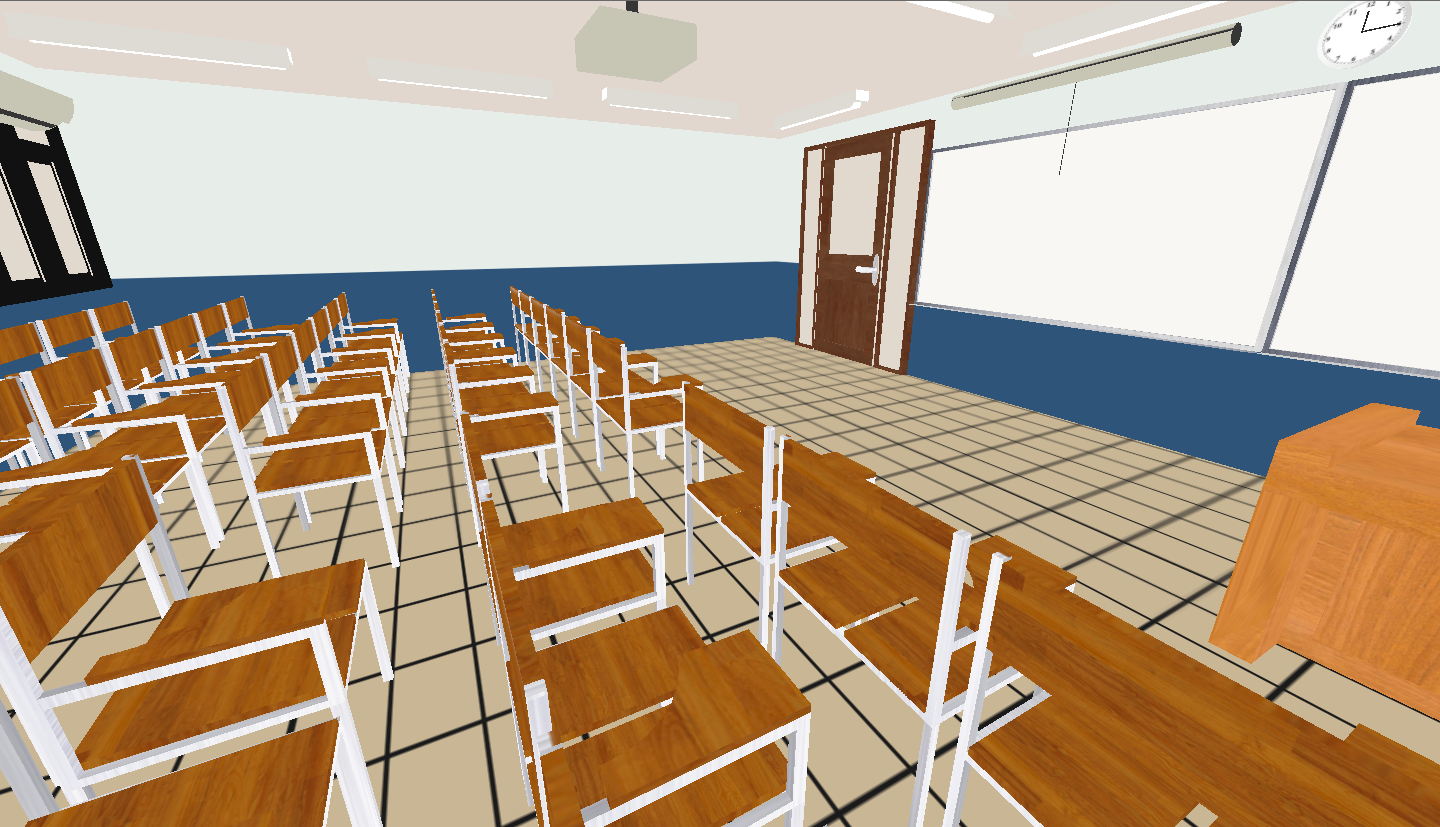
\includegraphics[scale=0.25]{kelas1}
			\caption{Pemodelan ruangan belajar mengajar gedung sembilan lantai satu di Universitas Katolik Parahyangan (1).}
		\end{figure}
		\begin{figure}[H]
			\centering
			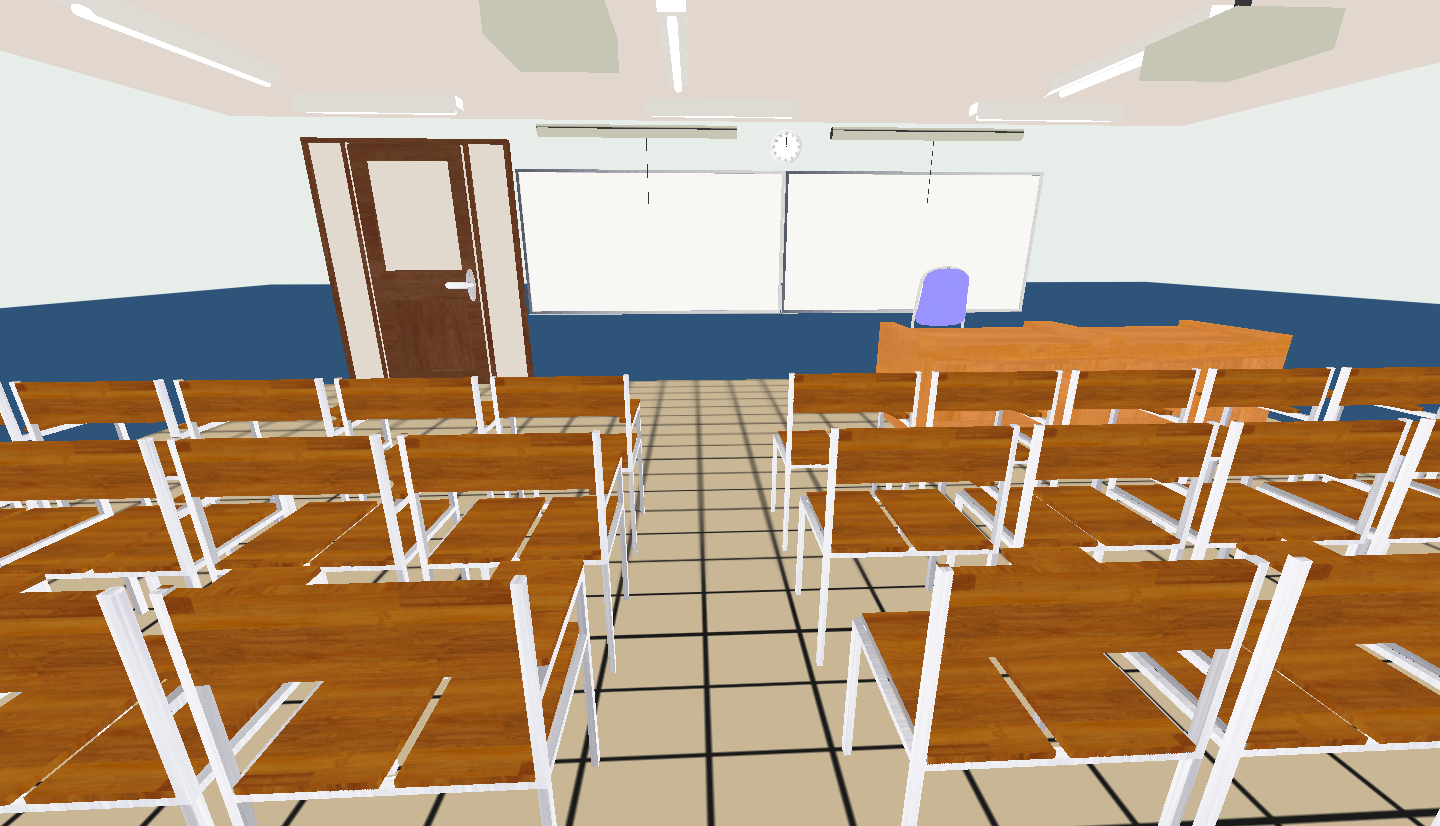
\includegraphics[scale=0.25]{kelas2}
			\caption{Pemodelan ruangan belajar mengajar gedung sembilan lantai satu di Universitas Katolik Parahyangan (2).}
		\end{figure}
		\begin{figure}[H]
			\centering
			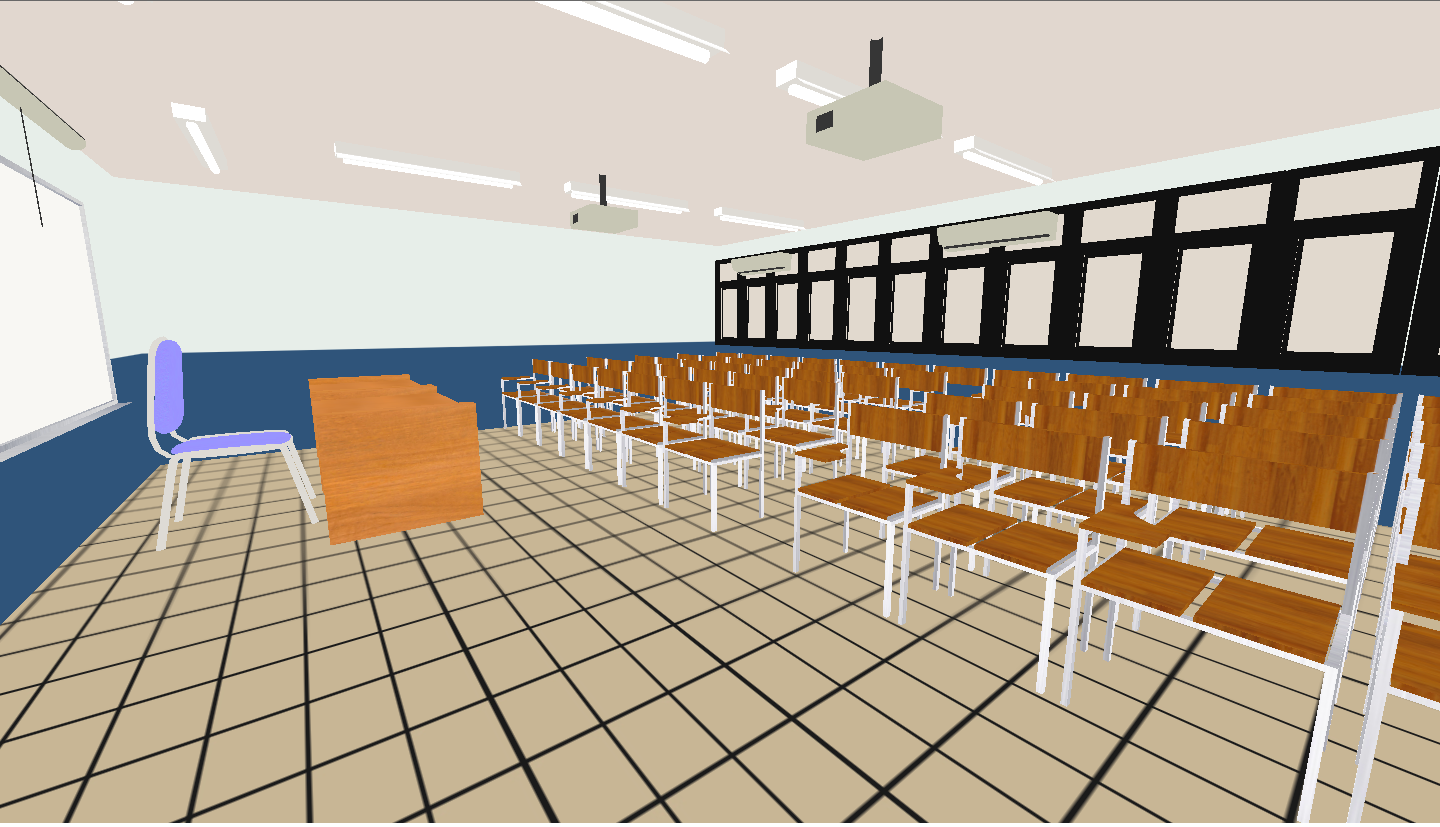
\includegraphics[scale=0.25]{kelas3}
			\caption{Pemodelan ruangan belajar mengajar gedung sembilan lantai satu di Universitas Katolik Parahyangan (3).}
		\end{figure}

		\item \textbf{Melakukan pengujian terhadap situs \textit{\textbf{web}} yang telah dibangun.} \\
		{\bf Status :} Ada sejak rencana kerja skripsi.\\
		{\bf Hasil :}

		\item \textbf{Menulis dokumen skripsi.}\\
		{\bf Status :} Ada sejak rencana kerja skripsi.\\
		{\bf Hasil :} Dokumen skripsi telah ditulis dari bab 1 sampai dengan bab 2. Pada bab 1 dibahas mengenai latar belakang, rumusan masalah, tujuan, batasan masalah, serta metodologi dan sistematika pembahasan. Bab 2 berisikan studi literatur tentang WebGL dan Pustaka Three.js.
		
	\end{enumerate}

\section{Pencapaian Rencana Kerja}
Persentase penyelesaian skripsi sampai dengan dokumen ini dibuat dapat dilihat pada tabel berikut :

\begin{center}
  \begin{tabular}{ | c | c | c | c | l | c |}
    \hline
    1*  & 2*(\%) & 3*(\%) & 4*(\%) &5* &6*(\%) \\ \hline \hline
    1    & 8 & 8 &  &  & 8 \\ \hline
    2    & 8 & 8 &  &  & 8 \\ \hline
    3    & 15 & 15 &  & &  10 \\ \hline
    4    & 6 & 6 &  & & 3 \\ \hline
    5    & 8 &  & 8 & & 3 \\ \hline
    6    & 30 &  & 30 & & 10 \\ \hline
    7    & 10 &  & 10 & &  \\ \hline
    8    & 15 & 3 & 12 & bab 1 dan 2 di S1 & 3 \\ \hline
    Total   & 100 & 40 & 60 & & 45 \\ \hline
   \end{tabular}
\end{center}

Keterangan (*)\\
1 : Bagian pengerjaan Skripsi (nomor disesuaikan dengan detail pengerjaan di bagian 5)\\
2 : Persentase total \\
3 : Persentase yang akan diselesaikan di Skripsi 1 \\
4 : Persentase yang akan diselesaikan di Skripsi 2 \\
5 : Penjelasan singkat apa yang dilakukan di S1 (Skripsi 1) atau S2 (skripsi 2)\\
6 : Persentase yang sidah diselesaikan sampai saat ini 

\section{Kendala yang dihadapi}
%TULISKAN BAGIAN INI JIKA DOKUMEN ANDA TIPE A ATAU C

\vspace{1cm}
\centering Bandung, \tanggal\\
\vspace{2cm} \nama \\ 
\vspace{1cm}

Menyetujui, \\
\ifdefstring{\jumpemb}{2}{
\vspace{1.5cm}
\begin{centering} Menyetujui,\\ \end{centering} \vspace{0.75cm}
\begin{minipage}[b]{0.45\linewidth}
% \centering Bandung, \makebox[0.5cm]{\hrulefill}/\makebox[0.5cm]{\hrulefill}/2013 \\
\vspace{2cm} Nama: \pembA \\ Pembimbing Utama
\end{minipage} \hspace{0.5cm}
\begin{minipage}[b]{0.45\linewidth}
% \centering Bandung, \makebox[0.5cm]{\hrulefill}/\makebox[0.5cm]{\hrulefill}/2013\\
\vspace{2cm} Nama: \pemB \\ Pembimbing Pendamping
\end{minipage}
\vspace{0.5cm}
}{
% \centering Bandung, \makebox[0.5cm]{\hrulefill}/\makebox[0.5cm]{\hrulefill}/2013\\
\vspace{2cm} Nama: \pembA \\ Pembimbing Tunggal
}
\end{document}

